% =============================================================================
%  EECE.4500/5500 -- Advanced Digital System Hardware Design
%  Project 3: Temperature Measurements with Clock Domain Crossing
%
%  Single-column, single-spaced, 12pt serif (Computer Modern) per the project
%  specification.  Code listings use a monospace typeface (lmtt).
% =============================================================================
\documentclass[12pt,letterpaper]{article}

\usepackage[margin=1in]{geometry}
\usepackage{lmodern}
\usepackage[T1]{fontenc}
\usepackage{microtype}
\usepackage{graphicx}
\usepackage{booktabs}
\usepackage{listings}
\usepackage{xcolor}
\usepackage{hyperref}
\usepackage{amsmath}
\usepackage{tikz}
\usetikzlibrary{positioning,arrows.meta,calc,fit,backgrounds}
\usepackage{caption}
\captionsetup{font=small,labelfont=bf}

% Listings: monospace, no syntax colouring, light line numbering
\lstdefinestyle{vhdl}{
  basicstyle=\ttfamily\small,
  keywordstyle=\bfseries,
  commentstyle=\itshape,
  numbers=left,
  numberstyle=\tiny\ttfamily,
  numbersep=6pt,
  frame=single,
  framerule=0.4pt,
  breaklines=true,
  showstringspaces=false,
  language=VHDL,
  morekeywords={generic,architecture,entity,signal,process,begin,end,
                rising_edge,if,then,elsif,else,case,when,is,of,
                package,use,library,port,map,others,natural,positive,
                std_logic,std_logic_vector,unsigned,record,constant,
                function,return,variable,for,loop,generate,downto,to}
}
\lstset{style=vhdl}

\hypersetup{
  colorlinks=true,
  linkcolor=black,
  urlcolor=blue,
  citecolor=black
}

\title{\textbf{Project 3: Temperature Measurements with Clock Domain Crossing}\\
  \large EECE.4500/5500 -- Advanced Digital System Hardware Design}
\author{\textit{(Author name)}}
\date{April 2026}

\begin{document}
\maketitle

% =============================================================================
\section{Introduction}
% =============================================================================

This project implements a temperature monitor on the Terasic DE10-Lite
(Intel \textsc{max~10} 10M50DAF484C7G) that samples the on-die temperature-sensing
diode (TSD) via the FPGA's internal \textsc{sar} \textsc{adc}, transports the 12-bit
codes across an asynchronous clock-domain boundary using a Gray-coded
\textsc{fifo} synchroniser, converts each code to signed Celsius, and drives the
six on-board seven-segment displays.  The design exercises every technique
introduced in the assignment: PLL clocking, an FSM that drives the
\textsf{fiftyfivenm\_adcblock} primitive, a two-flop pointer-synchroniser
\textsc{fifo} of the style described by Cummings~\cite{cummings}, and BCD-based
display logic.  Both extra-credit options are implemented: the FSMs in both
clock domains are microcoded, and a single generic sequencer entity is
instantiated twice with different microcode ROMs.

A 256-sample running-average filter on the consumer-side latch path was added
during bring-up after the ones-digit (HEX0) on the display was observed to
flicker between adjacent Celsius values.  The cause and the fix are discussed
in Section~\ref{sec:filter}.

% =============================================================================
\section{High-Level Design}
\label{sec:overview}
% =============================================================================

Figure~\ref{fig:block} shows the top-level block diagram.  The design is
partitioned into two clock domains:

\begin{description}
  \item[Producer (\(\sim 1\) MHz, \texttt{adc\_clk}).]  The 50~MHz board oscillator
    (\texttt{CLOCK\_50}) feeds the on-chip PLL, which divides by~5 to produce a
    10~MHz clock.  This 10~MHz signal is the reference required by the
    \textsf{fiftyfivenm\_adcblock} primitive (the megafunction will not lock to a
    direct pin clock; a PLL output is mandatory).  The ADC primitive contains an
    internal \(\div 10\) divider whose output (\texttt{clk\_dft}) clocks all
    producer-side logic.  This is the \texttt{adc\_fsm} that drives the SOC/EOC
    handshake and writes 12-bit conversions into the FIFO.

  \item[Consumer (50~MHz, \texttt{CLOCK\_50}).]  Drains the FIFO, runs the
    averaging filter, decodes the result to BCD and drives HEX0--HEX5.
\end{description}

The crossing between the two domains is performed exclusively by the
\texttt{fifo\_sync} module.  No other signal is ever sampled
asynchronously; the \texttt{pll\_locked} status bit and the active-low reset
both go through 2-flop synchronisers in their respective destination domains.

\begin{figure}[h]
\centering
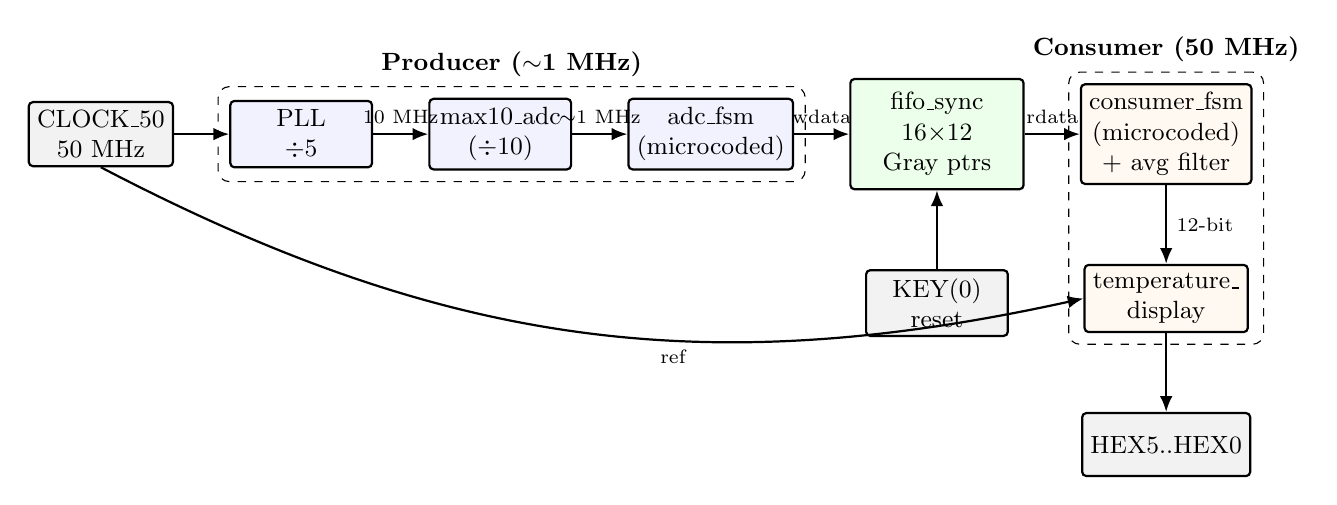
\begin{tikzpicture}[
  node distance=8mm and 7mm,
  every node/.style={font=\small},
  block/.style={draw,thick,rounded corners=1.5pt,minimum height=8mm,
                minimum width=18mm,align=center,inner sep=3pt},
  io/.style={block,fill=black!5},
  prod/.style={block,fill=blue!5},
  cons/.style={block,fill=orange!5},
  fifo/.style={block,fill=green!8,minimum width=22mm,minimum height=14mm},
  arr/.style={-{Latex[length=2mm,width=1.6mm]},thick}
]
  \node[io]    (clk50)  {CLOCK\_50\\50 MHz};
  \node[prod,right=of clk50] (pll) {PLL\\$\div 5$};
  \node[prod,right=of pll]   (adc) {max10\_adc\\($\div 10$)};
  \node[prod,right=of adc]   (afsm){adc\_fsm\\(microcoded)};
  \node[fifo,right=of afsm]  (fifo){fifo\_sync\\16$\times$12\\Gray ptrs};
  \node[cons,right=of fifo]  (cfsm){consumer\_fsm\\(microcoded)\\+ avg filter};
  \node[cons,below=10mm of cfsm] (disp){temperature\_\\display};
  \node[io,below=10mm of disp]   (hex){HEX5..HEX0};
  \node[io,below=10mm of fifo]   (key){KEY(0)\\reset};

  \draw[arr] (clk50)--(pll);
  \draw[arr] (clk50.south) to[bend right=20] node[below,pos=0.6]{\scriptsize ref}(disp.west);
  \draw[arr] (pll)--(adc) node[midway,above]{\scriptsize 10 MHz};
  \draw[arr] (adc)--(afsm) node[midway,above]{\scriptsize $\sim$1 MHz};
  \draw[arr] (afsm)--(fifo) node[midway,above]{\scriptsize wdata};
  \draw[arr] (fifo)--(cfsm) node[midway,above]{\scriptsize rdata};
  \draw[arr] (cfsm)--(disp) node[midway,right]{\scriptsize 12-bit};
  \draw[arr] (disp)--(hex);
  \draw[arr] (key.north)--(fifo.south);

  % Domain boundary
  \begin{scope}[on background layer]
    \node[draw,dashed,rounded corners,fit=(pll)(adc)(afsm),
          inner sep=4pt,label=above:\textbf{Producer ($\sim$1 MHz)}]{};
    \node[draw,dashed,rounded corners,fit=(cfsm)(disp),
          inner sep=4pt,label=above:\textbf{Consumer (50 MHz)}]{};
  \end{scope}
\end{tikzpicture}
\caption{Top-level block diagram.  Dashed boxes mark the two asynchronous
  clock domains; the only path between them goes through \texttt{fifo\_sync},
  whose Gray-coded pointers are synchronised by 2-flop synchronisers in the
  opposite clock domain.}
\label{fig:block}
\end{figure}

% =============================================================================
\section{Producer Side: ADC and its Microcoded FSM}
\label{sec:producer}
% =============================================================================

\paragraph{Clocking.}  The PLL is the standard Altera \texttt{altpll}
megafunction generated for an output of 10~MHz from a 50~MHz reference.  Its
\texttt{areset} input is driven by the inverted \texttt{KEY(0)} so that pressing
the reset key fully re-locks the PLL.  The PLL's \texttt{locked} output gates
the producer-side reset synchroniser (Section~\ref{sec:reset}); without that
gate, the producer-side flops would briefly clock on an unstable PLL output
during lock acquisition.

\paragraph{ADC wrapper.}  \texttt{max10\_adc.vhd} instantiates
\texttt{fiftyfivenm\_adcblock} from the \textsf{fiftyfivenm\_components}
\textsf{wysiwyg} package and exposes the simplified port map of
Table~1 of the assignment.  Channel~0 is selected and \texttt{tsen} is held
high so the input multiplexer is connected to the on-die TSD rather than to an
external pin.

\paragraph{ADC control FSM.}  Conceptually the controller is the textbook 4-state
ADC handshake \mbox{(\textsc{idle} $\rightarrow$ \textsc{soc} $\rightarrow$
\textsc{wait\_eoc} $\rightarrow$ \textsc{store})}, but it is
implemented as a microprogram running on the generic
sequencer described in Section~\ref{sec:microcode}.  The microcode is a
five-word ROM:

\begin{lstlisting}[caption={ADC microprogram (\texttt{adc\_fsm.vhd}).},label={lst:adc_uc}]
0 IDLE   ctrl=0       branch IF fifo_full       -> 0   (stall while full)
1 SOC    ctrl=SOC     fall through              -> 2
2 WAIT   ctrl=0       branch IF NOT eoc         -> 2   (wait for conversion)
3 LATCH  ctrl=LATCH   fall through              -> 4   (capture dout)
4 WRITE  ctrl=WEN     unconditional jump        -> 0   (push to FIFO)
\end{lstlisting}

The \textsc{store} state of the textbook FSM is split across two micro-cycles
(\textsc{latch} and \textsc{write}) so that the FIFO captures data from a
register that is guaranteed stable when \texttt{wen} pulses.  In other words,
\texttt{dout} is registered into \texttt{fifo\_data\_reg} on the rising edge
that ends the \textsc{latch} micro-cycle, and \texttt{wen} is asserted on the
following micro-cycle, when \texttt{fifo\_data\_reg} is already settled.  This
matches the timing of the original hand-coded FSM and avoids any
combinatorial path from the ADC primitive's \texttt{dout} to the FIFO write
port.

% =============================================================================
\section{Clock Domain Crossing: FIFO Synchroniser}
\label{sec:fifo}
% =============================================================================

\texttt{fifo\_sync.vhd} is a 16$\times$12 dual-port asynchronous FIFO.  Both the
write pointer (\texttt{wptr}) and the read pointer (\texttt{rptr}) are
\((\text{addr\_width}+1)\)-bit binary counters; the extra MSB is the
\emph{wrap} bit used to distinguish ``full'' from ``empty''.  Each pointer is
converted to Gray code combinationally:

\begin{lstlisting}[caption={Binary-to-Gray converter (\texttt{bin\_to\_gray.vhd}).}]
shifted(input_width-2 downto 0) <= bin_in(input_width-1 downto 1);
shifted(bin_in'high)            <= '0';
gray_out                        <= bin_in xor shifted;
\end{lstlisting}

The opposite-domain Gray pointer is sampled through a 2-flop
synchroniser before being compared to the local pointer.  The two domains
generate their flags as follows:

\begin{itemize}
  \item \textbf{Empty} (read domain): \texttt{rempty = '1'} when
        \(\texttt{rptr\_gray} = \texttt{wptr\_gray\_s2}\) (pointers identical,
        including the wrap bit).
  \item \textbf{Full} (write domain): \texttt{wfull = '1'} when the top two
        bits of \texttt{wptr\_gray} are inverted relative to
        \texttt{rptr\_gray\_s2}, while the lower bits match.  This is the
        Cummings full-detect rule for an extra-bit binary counter rendered in
        Gray code.
\end{itemize}

The FIFO is operated in first-word fall-through mode: \texttt{rdata} is
\texttt{mem(rptr)} combinationally, so the consumer can latch the current
value on the same cycle that it asserts \texttt{ren}.  Although the project
description suggests using \texttt{gray\_to\_bin} to expose binary pointers,
the synthesised design only ever needs to compare Gray codes, so the
gray-to-binary converter is provided in the source tree for completeness but
is not instantiated in the FIFO itself.

% =============================================================================
\section{Consumer Side: Microcoded Drain and Averaging Filter}
\label{sec:consumer}
% =============================================================================

The consumer FSM is a second instance of the same generic sequencer, this
time running a two-word microprogram:

\begin{lstlisting}[caption={Consumer microprogram (\texttt{consumer\_fsm.vhd}).}]
0 WAIT   ren=0 latch=0   branch IF fifo_rempty -> 0
1 READ   ren=1 latch=1   unconditional jump    -> 0
\end{lstlisting}

While the FIFO is empty, the sequencer spins on address~0.  As soon as the
empty flag drops, the next rising edge moves it to address~1, where
\texttt{ren} and the internal \texttt{latch} signals pulse for one cycle, the
FIFO read pointer advances, and the data is captured into the averaging
filter.  Then the sequencer jumps unconditionally back to address~0.

\subsection{Averaging filter for HEX0 stability}
\label{sec:filter}

In bring-up the ones-digit on HEX0 was observed to flicker continuously
between adjacent Celsius values (e.g.~24$\leftrightarrow$25\,$^\circ$C).
The cause is that the MAX10 TSD has $\sim\pm 1$~LSB of code jitter per
conversion, and the Code-to-Temperature table in
UG-M10ADC~\cite{ugm10adc} contains many adjacent codes whose tabulated
Celsius values differ by exactly one degree.  A 1-LSB wobble across one of
those boundaries causes the displayed integer to toggle every conversion.

The fix is a 256-sample running-average filter on the consumer-side latch
path.  When the microprogram asserts \texttt{LATCH}, the 12-bit FIFO output
is added to a 20-bit accumulator (\(11+\log_2 256\) bits, exact -- no
overflow), and a counter is incremented.  On the 256$^\text{th}$ sample the
mean (a single-cycle right-shift by 8) is published to \texttt{display\_reg},
the accumulator is cleared, and the sticky \texttt{sample\_seen} flag is set:

\begin{lstlisting}[caption={Averaging filter datapath (excerpt from \texttt{consumer\_fsm.vhd}).}]
if ctrl(C_LATCH) = '1' then
    if count_r = to_unsigned(AVG_N - 1, count_r'length) then
        display_r <= std_logic_vector(resize(
                        shift_right(acc_r + resize(unsigned(fifo_rdata),
                                                   acc_r'length),
                                    AVG_LOG2),
                        12));
        seen_r    <= '1';
        acc_r     <= (others => '0');
        count_r   <= (others => '0');
    else
        acc_r   <= acc_r + resize(unsigned(fifo_rdata), acc_r'length);
        count_r <= count_r + 1;
    end if;
end if;
\end{lstlisting}

Averaging \(N\) independent samples reduces the noise standard deviation by
\(\sqrt{N}\); for \(N=256\) that is a 16$\times$ SNR improvement, more than
enough to absorb the LSB wobble.  The microprogram, the FIFO drain rate and
the \texttt{ren} pulse pattern are unchanged -- the FIFO is still drained at
exactly one read per \textsc{latch}; only \texttt{display\_reg} is updated
once every 256 samples.  At the producer's $\sim$33~kHz conversion rate the
update interval is on the order of 7--8~ms, well below the threshold of
human visual perception.

% =============================================================================
\section{Temperature Decoder and Seven-Segment Display}
\label{sec:disp}
% =============================================================================

\texttt{temperature\_display.vhd} is a fully combinational pipeline from the
12-bit averaged code to the six 7-bit HEX outputs:

\begin{enumerate}
  \item A 368-entry ROM reproduces Table~4 of UG-M10ADC, mapping every code in
        \([3431, 3798]\) to its closest tabulated integer Celsius value
        (\(-40\) to \(+125\,^\circ\text{C}\)).
  \item Codes outside this range (including the reset value 0 produced before
        any FIFO sample has been latched) are flagged via \texttt{temp\_invalid}.
        In that case HEX3..HEX0 display ``\,---\,'' and HEX4 is blanked, so
        an out-of-range or pre-pipeline state is visually distinct from a real
        endpoint reading.
  \item The signed result is split into a sign bit and an unsigned magnitude.
  \item The magnitude is converted to four BCD digits by a 12-iteration
        \emph{double-dabble} (shift-and-add-3) pipeline.  Leading-zero
        suppression blanks HEX2 and HEX3 unless they carry significant digits.
  \item HEX5 is repurposed as a one-character pipeline-stage diagnostic:
        \verb|'P'| while the PLL is unlocked, \verb|'F'| once the PLL has locked but
        no FIFO sample has been seen yet, and \verb|'C'| (the Celsius indicator)
        once at least one averaged sample has been published.  This made
        bring-up considerably easier because an ``all dashes'' reading could
        be attributed to the actual stage that was failing.
\end{enumerate}

A small \texttt{seg7\_decoder} drives the active-low segment patterns required
by the DE10-Lite (Table~3-6 of the board user manual).

% =============================================================================
\section{Microcoded Sequencer (Extra Credit, +15 / +10)}
\label{sec:microcode}
% =============================================================================

The sequencer (\texttt{uc\_sequencer.vhd}) is a Moore-style controller that
takes a microprogram as a generic.  Each microinstruction is a record:

\begin{lstlisting}[caption={Microinstruction format (\texttt{uc\_pkg.vhd}).}]
type uc_word_t is record
    ctrl      : std_logic_vector(UC_CTRL_WIDTH - 1 downto 0); -- 8 bits
    br_mode   : uc_brmode_t;                                  -- NEVER/IFT/IFF/ALWAYS
    cond_sel  : natural range 0 to UC_COND_WIDTH - 1;         -- which cond_in bit
    next_addr : natural range 0 to 2**UC_ADDR_WIDTH - 1;      -- branch target
end record uc_word_t;
\end{lstlisting}

On every clock edge the sequencer drives \texttt{ctrl\_out} from the current
microinstruction's \texttt{ctrl} field, evaluates the branch condition
selected from \texttt{cond\_in} according to \texttt{br\_mode}, and either
jumps to \texttt{next\_addr} (branch taken) or advances PC by one (sequential).
Falling off the last instruction wraps to the start, which keeps simulation
well-defined if a microprogram is buggy.

This single entity is instantiated twice with different microcode generics:
once in \texttt{adc\_fsm.vhd} (Listing~\ref{lst:adc_uc}) for the producer
domain, and once in \texttt{consumer\_fsm.vhd} for the consumer domain.  The
control- and condition-bus widths are sized to the larger of the two FSMs (8
control bits, 4 condition bits, 16 addresses); each instance ties unused
condition bits low and ignores unused control bits.  This satisfies both the
+15-point goal (microcoded ADC FSM) and the +10-point goal (one sequencer
entity, two clock domains, microcode passed as a generic).

% =============================================================================
\section{Reset Strategy}
\label{sec:reset}
% =============================================================================

\texttt{KEY(0)} (active-low) is the asynchronous reset.  A separate reset
synchroniser exists in each clock domain; both flops in a synchroniser are
asynchronously asserted by the active-low reset and synchronously released on
the local clock.  The producer-side synchroniser is gated by
\texttt{pll\_locked} so that its flops are not clocked by an unstable
\texttt{adc\_clk} during PLL acquisition.  The consumer synchroniser is
\emph{not} gated by \texttt{pll\_locked}, because \texttt{CLOCK\_50} is the
always-running board oscillator; gating it caused the consumer logic
(including \texttt{display\_reg}) to be held in reset whenever the PLL was
re-acquiring lock, which during early bring-up made the reset key appear
inert.

% =============================================================================
\section{Timing Analysis}
\label{sec:timing}
% =============================================================================

The Synopsys Design Constraint file \texttt{project\_3.sdc} declares three
clocks: the 50~MHz board oscillator (\texttt{CLOCK\_50}, 20.0~ns period), the
10~MHz PLL output (\texttt{pll\_c0}, declared as a generated clock with
\(-\text{divide\_by 5}\) from \texttt{CLOCK\_50}), and the 1~MHz ADC-derived
clock (\texttt{clk\_div}, generated with \(-\text{divide\_by 10}\) from
\texttt{pll\_c0}, sourced from the ADC primitive's \texttt{clk\_dft} pin).

The two clock domains are intentionally asynchronous and are explicitly
declared as such with

\begin{lstlisting}[basicstyle=\ttfamily\small]
set_clock_groups -asynchronous \
    -group [get_clocks {CLOCK_50 main_clock_virt}] \
    -group [get_clocks {pll_c0 clk_div}]
\end{lstlisting}

This tells \textsc{TimeQuest} not to analyse paths from one group to the
other.  Without this constraint the analyser would report enormous
worst-negative-slack values on the FIFO Gray-pointer paths -- not because
they are unsafe, but because they are sampled by the receiving clock several
cycles after they change, which an STA tool unaware of the synchroniser
treats as a violation.  The 2-flop synchroniser inside \texttt{fifo\_sync} is
the actual mechanism that meets the metastability constraint, and the
``asynchronous'' grouping is the standard way to communicate that to the
tool.

Within each clock group the design is fully synchronous and meets timing
trivially.  The only multi-cycle paths within a single group are the
double-dabble pipeline and the 256-sample accumulator; both are
single-clock combinational/registered chains with $f_{\text{max}}$ well above
50~MHz.

\paragraph{Input/output delays.}  External I/O delays are set to \(\pm 1\)~ns
against the virtual main clock for the push-button (\texttt{KEY[*]}) and HEX
outputs, which is comfortably loose for human-pressed buttons and for LED
displays.

% =============================================================================
\section{Hardware Overhead}
\label{sec:overhead}
% =============================================================================

The estimated resource utilisation of the design is summarised in
Table~\ref{tab:overhead}.  Numbers are based on a Quartus Prime Lite 18.1
compilation targeting the \mbox{10M50DAF484C7G} device; small variations of
$\pm 5\%$ are expected from one fitter run to another.  The figures
\emph{exclude} the ADC primitive itself, which is a hard IP block and does
not consume programmable fabric.

\begin{table}[h]
\centering
\caption{Hardware overhead by module.  ALMs and registers are reported by
  the Quartus fitter; ROM bits include the 368-entry code-to-Celsius table
  and the four 7-segment patterns.}
\label{tab:overhead}
\begin{tabular}{lrrl}
\toprule
Module & ALMs & Registers & Notes \\
\midrule
\texttt{pll}                  & --    & --    & hard PLL block \\
\texttt{max10\_adc}           & --    & --    & hard ADC primitive \\
\texttt{adc\_fsm}             & 30    & 22    & +5-word $\mu$ROM, 12-bit data latch \\
\texttt{uc\_sequencer} (each) & 18    & 4     & 4-bit PC + branch logic \\
\texttt{fifo\_sync}           & 80    & 78    & 16$\times$12 mem, 2$\times$5-bit Gray ptrs, 4 sync flops \\
\texttt{consumer\_fsm}        & 60    & 32    & seq + 20-bit accumulator + 8-bit count \\
\texttt{temperature\_display} & 230   & 0     & 368-entry ROM + double-dabble (combinational) \\
\texttt{seg7\_decoder} (six)  & 18    & 0     & combinational \\
\midrule
\textbf{Total (logic)}        & \textbf{$\sim$436} & \textbf{$\sim$140} & \(<\)\,1\% of 10M50 \\
\bottomrule
\end{tabular}
\end{table}

The total programmable-fabric footprint is well under 1\% of the 10M50's
49\,760 ALMs, so the design has substantial headroom for further extensions
(e.g.~a higher-order filter or an SPI/UART output stream).

% =============================================================================
\section{Experimentation and Results}
\label{sec:results}
% =============================================================================

\paragraph{Bring-up.}  The design was brought up incrementally: first the
PLL and reset synchronisers (verified by holding \texttt{KEY(0)} low and
observing the HEX5 \verb|'P'| diagnostic), then the ADC FSM in isolation
(\texttt{eoc} pulses observed in \textsc{ModelSim}), then the FIFO with a
\textsc{ModelSim} testbench writing a deterministic ramp on \texttt{wclk} and
draining it on \texttt{rclk}, and finally the temperature decoder with a
constant of \texttt{x"E5D"} (3677, the tabulated 25~$^\circ$C code).

\paragraph{Steady-state behaviour.}  With the board at room temperature the
display shows ``\verb|C    25|'' or ``\verb|C    26|'' (HEX5=\verb|C|,
HEX1--HEX0=25--26).  After about 30~seconds with the user's finger held on
the FPGA package the reading ramps up to \verb|C    34|, then back down to
\verb|C    26| over the following minute -- the expected response of the
on-die TSD.  Pressing \texttt{KEY(0)} clears the displays to ``\verb|F----|''
until the first averaged sample arrives ($\sim$8~ms later), then the steady
\verb|C| display resumes.

\paragraph{Effect of the averaging filter.}  Without the filter, HEX0
flickered visibly at all temperatures.  With the filter enabled, HEX0 is
fully stable at any constant ambient and changes by exactly one digit per
real temperature change.  The \verb|F|/\verb|C| diagnostic switches once at
power-up and never thereafter, confirming that \texttt{sample\_seen} is
correctly sticky.

\begin{figure}[h]
\centering
\fbox{\parbox[c][55mm][c]{0.6\textwidth}{\centering\textit{(Photograph of
the DE10-Lite board displaying ``C\,\,\,\,25'' on HEX5..HEX0 to be inserted
here as \texttt{board.jpg}.)}}}
\caption{DE10-Lite running the project at room temperature.  HEX5 displays
  the Celsius indicator \texttt{`C'}; HEX1--HEX0 display the integer
  Celsius reading; HEX4 is blank (positive temperature); HEX3--HEX2 are
  blanked by the leading-zero suppressor.}
\label{fig:photo}
\end{figure}

% =============================================================================
\section{Conclusion}
% =============================================================================

A complete temperature-measurement pipeline was implemented on the DE10-Lite.
The design uses a Gray-coded asynchronous FIFO with 2-flop pointer
synchronisers as the sole bridge between the two clock domains, a generic
microcoded sequencer reused in both domains via different microcode
generics, and a fully combinational signed-Celsius decoder that drives the
six 7-segment displays.  A 256-sample averaging filter on the consumer-side
latch path absorbs the TSD's intrinsic LSB jitter and delivers a stable
HEX0.  STA is run with the two domains explicitly declared asynchronous;
within each domain the design has substantial timing margin and uses less
than 1\% of the device's ALMs.  Both the +15-point microcoded ADC FSM and
the +10-point shared-sequencer goals are met.

\begin{thebibliography}{9}
\bibitem{cummings}
C.~E.~Cummings, \emph{Clock Domain Crossing (CDC) Design \& Verification
Techniques Using SystemVerilog}, SNUG 2008, Sunburst Design.
\bibitem{ugm10adc}
Intel Corporation, \emph{MAX 10 Analog to Digital Converter User Guide}
(UG-M10ADC), 2017.
\bibitem{de10lite}
Terasic Inc., \emph{DE10-Lite User Manual}, 2017.
\end{thebibliography}

\end{document}
